\newpage
\subsection{View}
Sofern nicht anders angebeben sind alle Klassen in diesem 
\\Unterkapitel React-Komponenten.

\begin{landscape}
    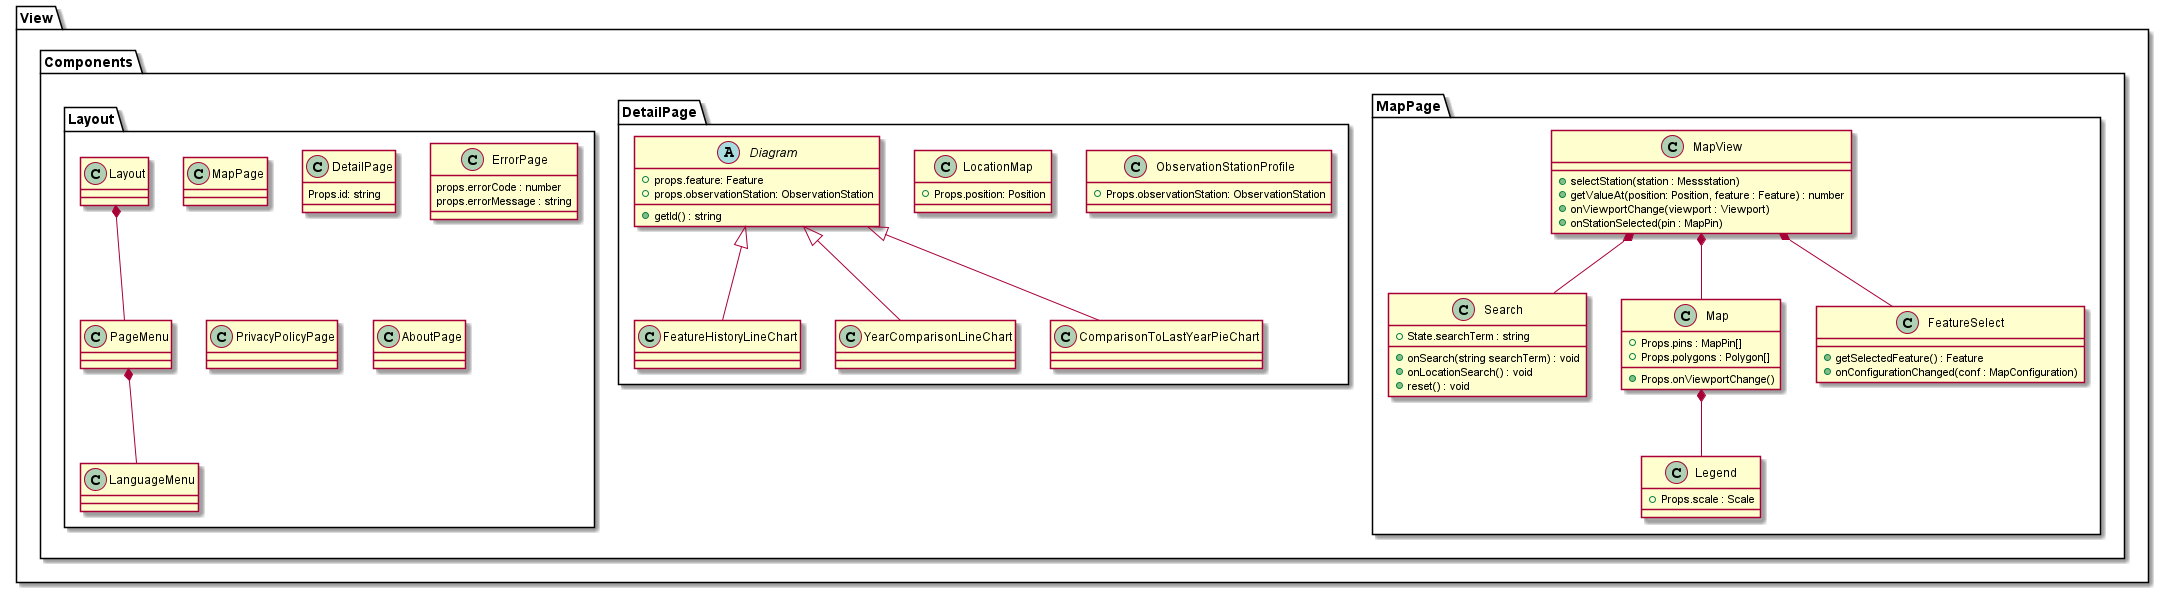
\includegraphics[height=6cm]{MVC/View/View.png}
\end{landscape}


\subsubsection{Layout}
\begin{Class}{Layout}
    Die Hauptkomponente der Anwendung. Zeigt das Seitenmenü und Anwendungsleiste an.
    Je nach Routing werden weitere Komponenten geladen.
\end{Class}

\begin{Class}{LanguageMenu}
    Eine Auswahlkomponente für Sprachen.
    Benötigt keine Attribute da die statische Language Klasse genutzt wird.
\end{Class}

\begin{Class}{AboutPage}
    Zeigt das Impressum in der gewählten Sprache an.
\end{Class}

\begin{Class}{PrivacyPolicyPage}
    Zeigt die Datenschutzerklärung in der gewählten Sprache an.
\end{Class}

\begin{Class}{ErrorPage}
    Wird bei einem kritischen Fehler aufgerufen.
    Zeigt eine Fehlermeldung an und enthält einen Button der auf die Kartenseite führt.
    \bigskip\\
    \textbf{Attribute}
    \begin{itemize}
        \item \texttt{Props.errorCode}
        \\ Ein Fehlercode.
        \item \texttt{Props.errorMessage}
        \\ Der Sprachdateien-Schlüssel für die Fehlermeldung.
    \end{itemize}
\end{Class}

\subsubsection{MapPage.Components}
    \begin{Class}{MapPage}
        Die Hauptkomponente der Kartenansicht. Enthält \emph{MapView}.
    \end{Class}
    \begin{Class}{MapView}
        Eine Komponente die die Karte selbst und weitere Steuerelemente wie die Suche, Konfiguration und Legende beinhaltet.
        \bigskip\\
        \textbf{Methoden}
        \begin{itemize}
            \item \texttt{selectStation(station : ObservationStation)}
            \\ Legt die angegebene ObservationStation als ausgewählt fest.
            \item \texttt{getValueAt(position: Position, feature : Feature) : float}
            \\ Berechnet mithilfe naher Messstationen einen Schätzwert des gewählten Features an einer bestimmter Position.
            \\ Rückgabe:
            \\ \emph{null}: Es konnte kein Wert bestimmt werden da der Punkt zu weit entfernt von Messstationen ist.
            \\ \emph{float}: Der geschätzte Wert
            \item \texttt{onViewportChange(viewport : Viewport)}
            \\ Verarbeitet die Änderung des Viewports und aktualisiert die Pins und Polygone auf der Karte.
            \item \texttt{onStationSelected(pin : MapPin)}
            \\ Verarbeitet den Klick auf einen Stations-Marker und aktualisiert das zugehörige Popup.
        \end{itemize}
    \end{Class}

    \begin{Class}{FeatureSelect}
        Eine Komponente für Einstellungen der Karte.
        \bigskip\\
        \textbf{Methoden}
        \begin{itemize}
            \item \texttt{getSelectedFeature() : Feature}
            \\ Rückgabe:
            \\ \emph{null}: Fehler, nicht definiert
            \\ \emph{Feature}: aktuell ausgewähltes Feature
            \item \texttt{onConfigurationChange(conf: MapConfiguration)}
            \\ Wird aufgerufen wenn sich aus einer Aktion des Nutzers eine neue Kartenkonfiguration ergibt.
        \end{itemize}
    \end{Class}

    \begin{Class}{Search}
        Ein Suchfeld für Adressen und ein Button zur automatischen Positionserkennung.
        \bigskip\\
        \textbf{Methoden}
        \begin{itemize}
            \item \texttt{onSearch(string searchTerm) : void}
            \\ Wird aufgerufen wenn auf den Such-Button geklickt wird.
            \\ Es wird nach der Adresse gesucht und das entsprechende Event im MapController aufgerufen.
            \item \texttt{onLocationSearch() : void}
            \\ Wird bei Klick auf den "Lokalisieren" Knopf aufgerufen und ruft die entsprechende Methode im MapController auf.
            \item \texttt{reset() : void}
            \\ Setzt searchTerm auf das leere Wort.
        \end{itemize}
        \textbf{Attribute}
        \begin{itemize}
            \item \texttt{searchTerm : string}
            \\ Der aktuelle Inhalt der Textbox der Komponente.
        \end{itemize}
    \end{Class}
    
    \begin{Class}{Map}
        Eine Leaflet-Karte mit anpassbaren Markern und Polygonen.
        \bigskip\\
        \textbf{Methoden}
        \begin{itemize}
            \item \texttt{Props.onViewportChanged(viewport : Viewport)}
            \\ Wird aufgerufen wenn die Leaflet-Karte verschoben wird.
            \item \texttt{Props.handlePopup(pin : MapPin)}
            \\ Wird aufgerufen wenn ein Marker angeklickt wird.
        \end{itemize}
        \textbf{Attribute}
        \begin{itemize}
            \item \texttt{Props.pins : MapPin[]}
            \\ Die Marker die auf der Karte angezeigt werden sollen.
            \item \texttt{Props.polygons : Polygon[]}
            \\ Die Polygone die auf der Karte angezeigt werden sollen.
        \end{itemize}
    \end{Class}
    
    \begin{Class}{Legend}
        Eine Legende für die Farben der aktuellen Ansicht.
        \bigskip\\
        \textbf{Attribute}
        \begin{itemize}
            \item \texttt{Props.scale : Skala}
            \\ Die aktuell verwendete Skala.
        \end{itemize}
    \end{Class}
    
    \begin{Class}{StationInfo}
        Das Popup für eine bestimmte Messstation. Es beinhaltet Metadaten und einen Button zur Detailseite.
        \bigskip\\
        \textbf{Attribute}
        \begin{itemize}
            \item \texttt{openDetails : MaterialUI.Button}
            \\ click() öffnet die Detailansicht mit der ID der \emph{station}
            \item \texttt{Props.station : ObservationStation}
            \\ Die Messstation zu der die StationInfo gehört.
        \end{itemize}
    \end{Class}

    \begin{Class}{FeatureInfo}
        Popup, das weitere Informationen über das auf der \gls{Kartenansicht} gewählte Feature anzeigt.
        \bigskip\\
        \textbf{Attribute}
        \begin{itemize}
            \item \texttt{Props.feature: Feature}
            \\Das gewählte Feature.
        \end{itemize}
    \end{Class}

\subsubsection{DetailPage}
    \begin{Class}{<<abstract>> Diagram}
        Ein Diagramm, dass verschiedene Daten visualisiert. Ein Diagramm Hat eine Überschrift, eine Erklärung, und eine GoogleCharts Chart. Die Klasse fragt ihre dargestellten Daten selbstständig beim Rendern vom DataProvider an.
        \bigskip\\
        \textbf{Attribute}
        \begin{itemize}
            \item \texttt{Props.observationStation: ObservationStation}
            \item \texttt{Props.feature: Feature}
        \end{itemize}
        \textbf{Methoden}
        \begin{itemize}
            \item \texttt{getId(): number}
            \\Gibt die Id des Diagramms zurück.
        \end{itemize}
        

    \end{Class}

    \begin{Class}{LocationMap}
        Eine Karte, die eine Position anzeigt.
        \bigskip\\
        \textbf{Attribute}
        \begin{itemize}
            \item \texttt{Props.position: Position}
        \end{itemize}
    \end{Class}

    \begin{Class}{ObservationStationProfile}
        Steckbrief einer ObservationStation, die den Namen, die Position, die Beschreibung und die letzten Messwerte einer ObservationStation anzeigt.
        \bigskip\\
        \textbf{Attribute}
        \begin{itemize}
            \item \texttt{props.observationStation: ObservationStation}
        \end{itemize}
    \end{Class}

    \begin{Class}{FeatureHistoryLineChart implements Diagram}
        Diagramm, dass die Messwerte eines Features über einen gewählten Zeitraum anzeigt. Dieses Dieagramm bietet die die Auswahl mehrerer Zeiträume.
    \end{Class}

    \begin{Class}{YearComparisonLineChart implements Diagram}
        Liniendiagramm, dass mit verschiedenen Graphen den Jahresverlauf der Messwerte eines Features von verschiedenen Jahren visualisiert.
    \end{Class}

    \begin{Class}{ComparisonToLastYearPieChart implements Diagram}
        Tortendiagramm, dass anzeigt, an wie vielen Tagen des letzten Jahres der Messwert eines Features zu vergleichbarer Uhrzeit höher bzw. niedriger war als der derzeitige Messwert.
    \end{Class}


